\documentclass[journal,onecolumn, 9pt]{IEEEtran}
\usepackage[left=1.5cm,right=1.5cm,top=1.5cm,bottom=1.5cm]{geometry}
\usepackage[utf8]{inputenc}
\usepackage[english]{babel}
\usepackage{minted}
\setminted{fontsize=\small}
\usepackage{booktabs}
\usepackage{amsmath}
\usepackage{float}
\usepackage{mathtools}
\usepackage{color}
\usepackage{amsthm}
\usepackage{parskip}
\usepackage{graphicx}
\usepackage{epstopdf}
\usepackage{amssymb}
\usepackage{mathrsfs}

\newcommand{\subparagraph}{}
\usepackage[compact]{titlesec}

\titlespacing{\section}{0pt}{\parskip}{-\parskip}
\titlespacing{\subsection}{0pt}{\parskip}{-\parskip}
\titlespacing{\subsubsection}{0pt}{\parskip}{-\parskip}

\usepackage{subcaption}


\usepackage[backend=biber, style=trad-abbrv]{biblatex}
\makeatletter
\def\blx@maxline{77}
\makeatother

%\linespread{0.9}

\usepackage{pgfplots}
\pgfplotsset{compat=newest}
\usepgfplotslibrary{groupplots}
\usepgfplotslibrary{dateplot}
\usepackage{tikzscale}

\theoremstyle{definition}
\newtheorem{defn}{Definition}[section]

\usepackage[binary-units=true]{siunitx}

\newcommand{\py}[1]{\mintinline{python}{#1}}
\newcommand{\java}[1]{\mintinline{java}{#1}}
\newcommand{\sql}[1]{\mintinline{sql}{#1}}
\newcommand{\scala}[1]{\mintinline{scala}{#1}}

\renewcommand{\epsilon}{\varepsilon}
\renewcommand{\theta}{\vartheta}
\renewcommand{\kappa}{\varkappa}
\renewcommand{\rho}{\varrho}
\renewcommand{\phi}{\varphi}

\newcommand{\db}{\mathcal{D}}
\newcommand{\is}{\mathcal{I}}
\newcommand{\tr}{\mathcal{T}}

\newcommand{\abs}[1]{|#1|}

\usepackage{hyperref}

\usepackage{csquotes}

\title{Languages \& translators: Domain-specific languages}
\author{Gilles Peiffer (24321600), Liliya Semerikova (64811600)}
\date{May 15, 2020}

\begin{document}

\maketitle

\begin{abstract}
	This paper gives some more insight into the domain-specific language we designed for the third project of LINGI2132.
	Several key design choices are explained, and more information is given about the strengths and weaknesses of our implementation.
	We also briefly cover possible further improvements which one could make to the DSL in order to enable more functionality or improve performance/readability.
\end{abstract}

\section{Introduction}
Domain-specific languages (DSL) are an interesting branch of programming language design that has been getting a lot of attention in the literature recently.
Many general-purpose languages (GPL) are not suited to the specificities of several domains, and the ability to add custom language constructs to an existing language has a large amount of pull on software engineers choosing a language for their project.
One GPL allowing the use of DSLs is Scala, which is based on the JVM.
This paper contains the description of a proof-of-concept DSL called\footnote{Another possible name is ``\textbf{SC}ala-in\textbf{H}erited \textbf{A}id for \textbf{U}ser-defined \textbf{S}oftware'', or ``\textbf{SCHAUS}'' for short.} ``\textbf{D}sl for \textbf{U}ltimate \textbf{BR}owser-based entert\textbf{A}inment functionalit\textbf{Y}'', or ``\textbf{DUBRAY}'' for short, which allows one to build simple browser-based games using Scala.js.

In order to do that, we developed a simple implementation of the well-known Snake game, which uses our DSL.
Section~\ref{sec:functionalities} gives an overview of the various functionalities of our DSL, with documented examples.
In Section~\ref{sec:evaluation}, we describe various strengths and weaknesses of our DSL.
Finally, Section~\ref{sec:improvements} gives various further improvements which could be make to extend the existing DSL with more functionality.
In order to prove the versatility of our DSL, we also wrote a game of Pong with it.

\section{Functionalities}
\label{sec:functionalities}
\subsection{First DSL}
Our DSL is heavily inspired from the DSL given in the first part of the project, which was based around various \scala{Shape}s (\scala{Rectangle} and \scala{Circle}) and how one could add them together into so-called ``\scala{ComposedShape}s'', containing a \scala{List} of \scala{Shape}s.

Several properties were defined for these \scala{Shape}s, such as their color, the stroke width with which they should be drawn, or geometric attributes such as the width, height and radius.

\subsection{Design Choices}
Our final DSL is based around entities called \scala{Spot}s, which represent an entity which can be drawn on a canvas.
Structurally, they are similar to the \scala{Shape}s of the previous exercise.
\scala{ComposedSpot}s and \scala{ComposedSpot2D}s are one-dimensional and two-dimensional arrays of \scala{Spot}s, and can be used to represent a group of related \scala{Spot}s (such as, for example, the body parts of a snake).

\subsection{List of Functionalities}
Our proof-of-concept DSL provides multiple different functionalities:
\begin{itemize}
	\item A vast library of \scala{Spot}s, which can be extended even further to accomodate game-specific spots (such as a spaceship for Space Invaders or an asteroid for Asteroids).
	\item An intuitive interaction with the keyboard, abstracted in \texttt{Keyboard.scala}.
	\item Utilities to combine \scala{Spot}s into lists or even matrices, with appropriate methods to operate on them.
	\item A simple and concise control structure designed specifically to deal with browser-based games, which enables one to easily switch between games while still maintaining useful properties such as easy displaying of game commands, seamless restarting of games, and concisely-written code.
	\item A set of operations on \scala{Spot}s which one can extend with ease to change the color, stroke width or font of text and images being drawn on screen, as well as the necessary methods to display this text/image.
	\item Native support for grid-based games.
	\item Extensive tests to verify correctness.
\end{itemize}

\subsection{Properties}
Many of the properties which make Scala well-suited for building DSLs were used, such as traits, monads, strong and static typing, type inference, implicits, currying, closures, custom flow control, etc.
Note that for brevity, some code extracts have been slightly modified.

\subsubsection{Traits}
Our implementation uses traits in order to define what a \scala{Spot} represents (in our case, it has a position, a \scala{move} method to change its position, and a \scala{change} method to change one its properties).
Additionally, a second trait is used to represent the attributes of a \scala{Spot}: \scala{SpotAttributes}, i.e. its color and stroke width.
\begin{minted}{scala}
sealed trait Spot {
	type A <: Spot
	val position: Point = Point(0, 0)
	def change(property: CanvasElementModifier[A]): Unit = ...
	def move(p: Point): Unit = ...
}
trait SpotAttributes {
	var color = "black"
	var strokeWidth = 1
	def color(col: String): Unit = color = col
	def strokeWidth(n: Int): Unit = strokeWidth = n
}
\end{minted}

Traits are also used when defining entities which modify these properties, so-called \scala{CanvasElementModifier}s, which must define a \scala{change} method as well.

\subsubsection{Monads}
\scala{ComposedSpot} defines a \scala{map} and \scala{flatMap} method, and is thus a monad.

\subsubsection{Strong/static Typing and Type Inference}
All throughout our code, explicit and implicit typing are used.
Scala requires one to use explicit types in some situations, such as function arguments, but in other places, where possible, the type is inferred at run-time.
Examples of this are shown in the listings above.
Our DSL also makes use of this in order to detect type mismatches.

\subsubsection{Implicits}
Implicits are used in our demo DSL to combine \scala{ComposedShape}s with different element types into one list with a common supertype (\scala{Shape}, in this case).
\begin{minted}{scala}
implicit def and[U <: Shape](shape: Array[U]): ComposedShape[Shape] = {
	ComposedShape(s.toList) and ComposedShape(shape.toList)
}
\end{minted}

\subsubsection{Currying}
In \scala{ComposedSpot2D}, the data is stored inside an array of arrays (functionally, this is thus equivalent to a two-dimensional matrix).
In order to allow nicer syntax when accessing the members of such a grid, we implemented currying, as follows (where \scala{spots} contains the matrix):
\begin{minted}{scala}
case class ArrayMapper(i: Int) {
	def apply(j: Int): Spot = spots(i)(j)
	...
}
def apply(i: Int): ArrayMapper = ArrayMapper(i)
\end{minted}
With this, elements of the grid can be accessed as such: \scala{grid.spots(i)(j)}.

\subsubsection{Closures}
Writing functional code is often simplified by the use of closures, as in the following example, which occurs when generalizing the \scala{GameLauncher} to work with all games.
\begin{minted}{scala}
val decision: () => Any = () =>
	if (!hasSeenCommands) keepWaiting()
	else if (game.alive) gameLoop()
	else reset()
\end{minted}
Often closures are also involved when using call-by-name parameters, as is the case in our code.

\subsubsection{Custom flow control}
The following example shows the use of our custom ``play with messages'' control structure:
\begin{minted}{scala}
play (SnakeGame) withMessages ("Arrow keys to move, space to play", "Press space to restart")
\end{minted}
Under the hood, this works very similarly to the \scala{onException} structure that was written during the second Scala practice session, with intermediate classes.

\subsection{Examples of Use}
Below, we give several examples of usage of the DSL.

\subsubsection{Defining a grid}
The following code extract defines a grid for the Snake game:
\begin{minted}{scala}
// Walls.
val wallTop = ComposedSpot(Array.tabulate(w)(i => Wall(Point(0, i), size)))
...
val wallLeft = ComposedSpot(Array.tabulate(h - 2)(i => Wall(Point(i + 1, w - 1), size)))
// Field; define the white squares that make up the playing field.
val field = ComposedSpot2D(Array.ofDim[Empty](h, w))
for (i <- 0 until h; j <- 0 until w) {
	field(i)(j) = Empty(Point(i + 1, j + 1), size)
}
field change Color(emptyColor)
// Define the grid, containing both the walls and the field.
val grid = Grid(w, h, wallTop, wallBottom, wallRight, wallLeft, field)
\end{minted}
We start by defining the walls, then the playing field (for which we use the \scala{change} method in order to color it in white), and finally the grid, which combines both.
It also shows an example of currying, in how the playing field is built.

\subsubsection{Defining a snake}
The following code extract shows how to define a snake, and how to make it appear on the grid.
\begin{minted}{scala}
// The snake (starts off at size 1, in the middle of the playing field).
val middle = Point((h - h%2) / 2, (w - w%2) / 2)
val snake = ComposedSpot[Snake](Array(Snake(middle, size)))
var direction = Point(1, 0) // Direction of the snake (initially, to the right).
grid.spots(middle.x.toInt)(middle.y.toInt) = snake.head
snake change Color(snakeColor)
\end{minted}
The snake should start off in the middle of the grid, moving to the right initially.
We also change its color to be green using the DSL.

\subsubsection{Showing Results in Pong}
The following code snippet shows how results are shown in our Pong implementation, using our DSL which enables one to easily show messages on screen.
\begin{minted}{scala}
// Scores of the players.
val score1 = Score(Point(35 * spotSize, 10 * spotSize), spotSize, 0)
val score2 = Score(Point(65 * spotSize, 10 * spotSize), spotSize, 0)
val message = Message(Point(50 * spotSize, 5 * spotSize), spotSize, "Score")
// Win messages.
val winMessage1 = Message(Point(50 * spotSize, 30 * spotSize), spotSize, "Player 1 wins!")
val winMessage2 = Message(Point(50 * spotSize, 30 * spotSize), spotSize, "Player 2 wins!")
val finalMessage = Message(Point(50 * spotSize, 40 * spotSize), spotSize, ending)
score1 change Font("15px Helvetica")
score2 change Font("15px Helvetica")
...
canvasy.showScore(score1)
canvasy.showScore(score2)
canvasy.showMessage(message)
...
if (score1.score > score2.score) canvasy.showMessage(winMessage1)
else canvasy.showMessage(winMessage2)
\end{minted}

\subsection{Screenshots}
Figure~\ref{fig:screenshots} shows some screenshots from the games we wrote using our DSL.
\begin{figure*}
	\centering
	\begin{subfigure}[t]{0.32\textwidth}
		\centering
		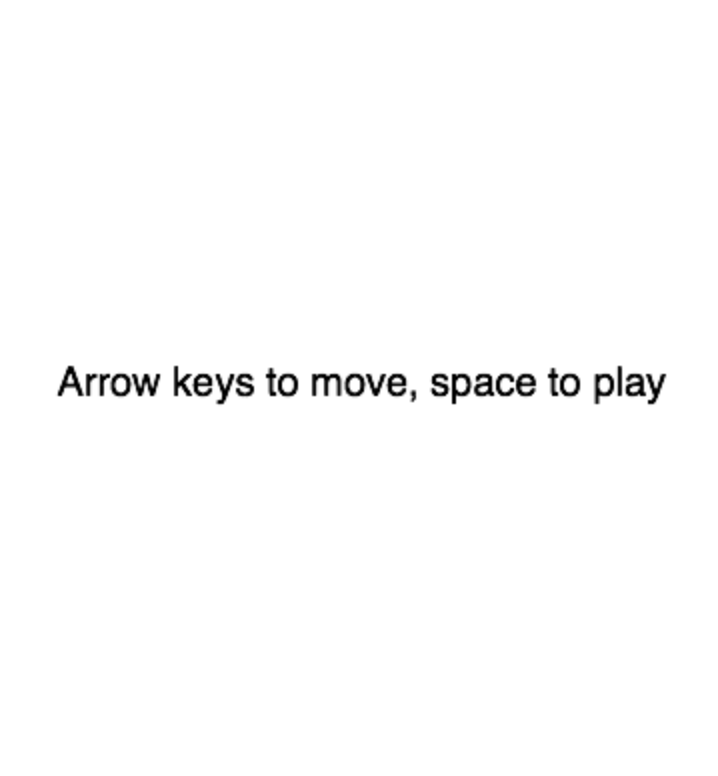
\includegraphics[width=\textwidth]{img/start_message.png}
		\caption{Start message explaining controls, waiting for user input (with custom message).}
		\label{fig:sc1}
	\end{subfigure}
	\hfill
	\begin{subfigure}[t]{0.32\textwidth}  
		\centering 
		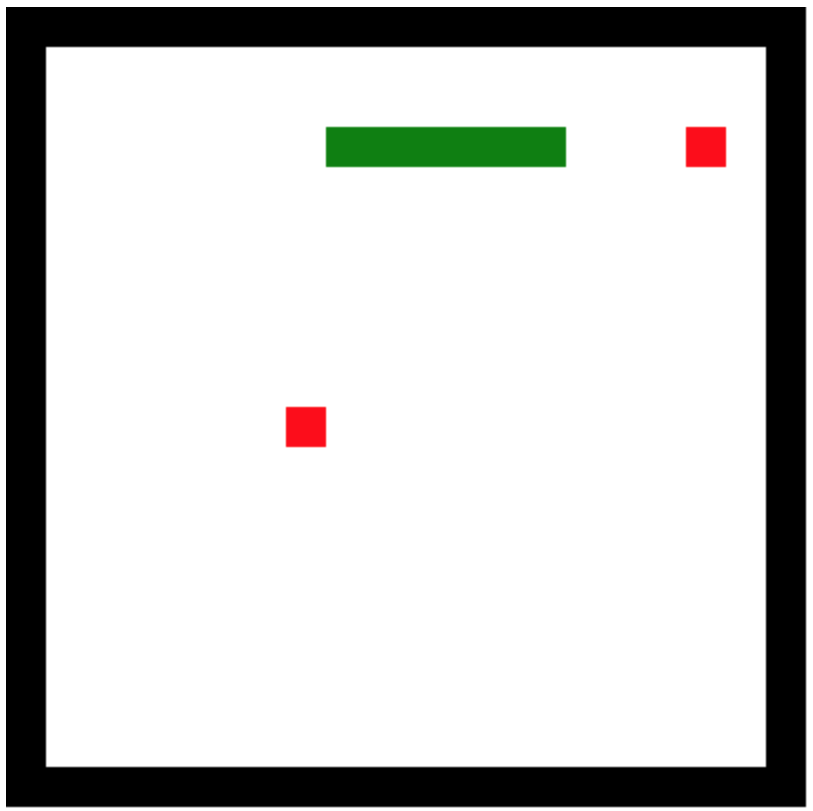
\includegraphics[width=\textwidth]{img/snake_gameplay.png}
		\caption{Playing a game of Snake.}
		\label{fig:sc2}
	\end{subfigure}
	\hfill
	\begin{subfigure}[t]{0.32\textwidth}   
		\centering 
		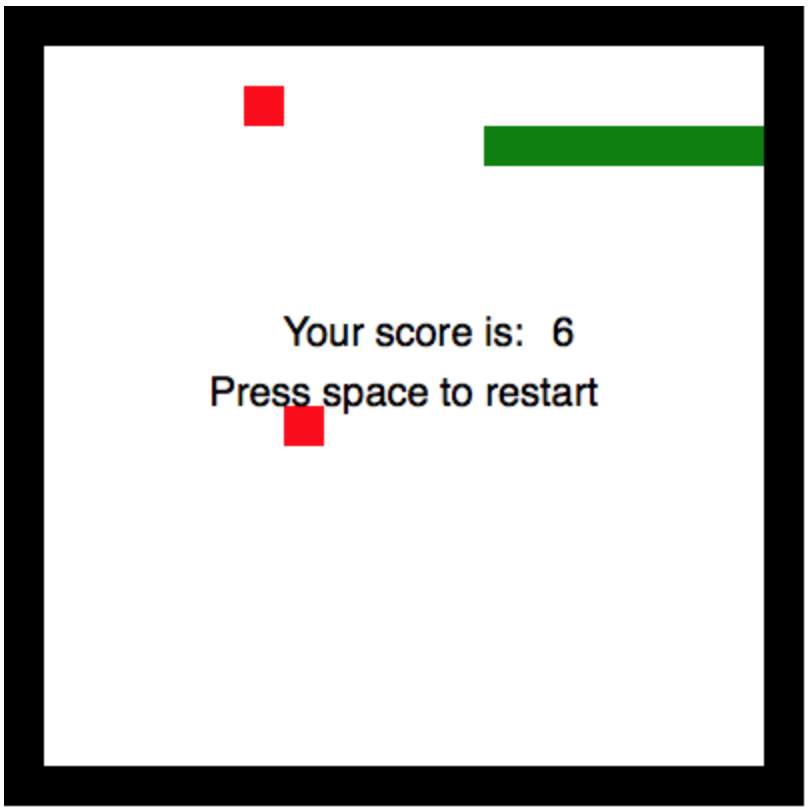
\includegraphics[width=\textwidth]{img/snake_end.png}
		\caption{End screen of a game of Pong, with custom restart message.}
		\label{sc3}
	\end{subfigure}
	\vskip\baselineskip
	{\hfill
	\begin{subfigure}[t]{0.32\textwidth}   
		\centering 
		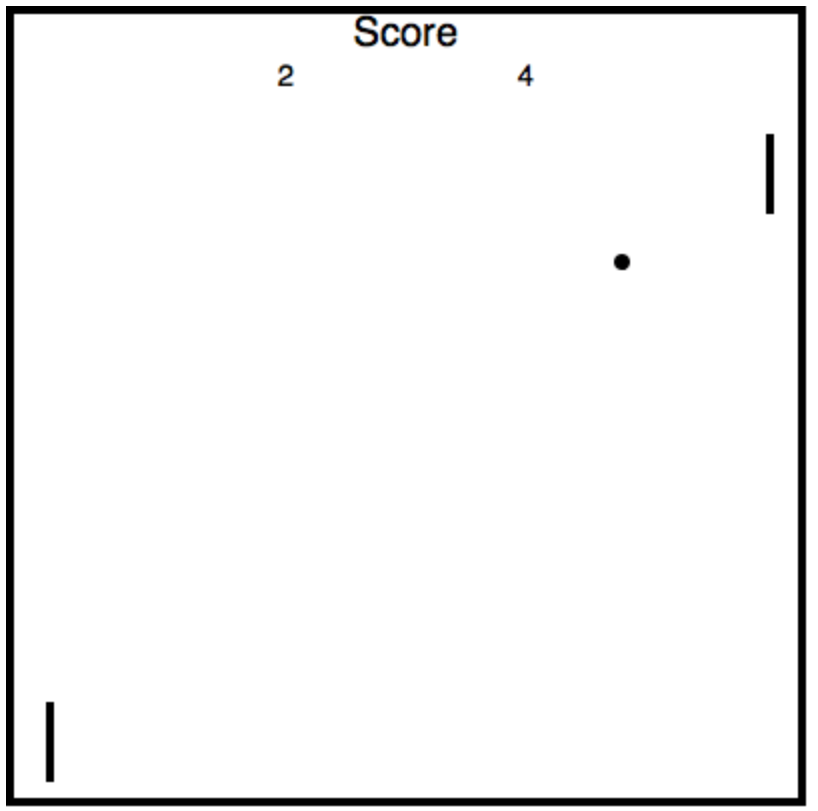
\includegraphics[width=\textwidth]{img/pong_gameplay}
		\caption{Playing a game of Pong.}
		\label{fig:sc4}
	\end{subfigure}
	\quad
	\begin{subfigure}[t]{0.32\textwidth}   
		\centering 
		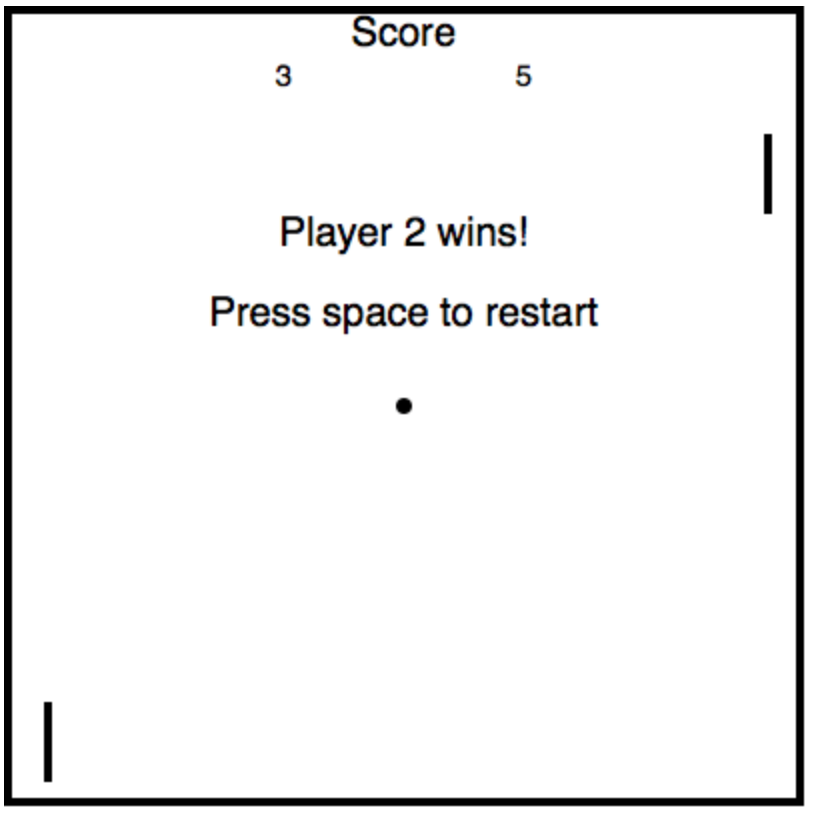
\includegraphics[width=\textwidth]{img/pong_end.png}
		\caption{End screen of a game of Pong, with custom restart message.}
		\label{fig:sc5}
	\end{subfigure}
	\hfill}
	\caption{Screenshots from the games we implemented.} 
	\label{fig:screenshots}
\end{figure*}

\section{Strengths and Weaknesses}
\label{sec:evaluation}
As building a good DSL is partially an art, there is no construction which is optimal from all points of view.
In our DSL, simplicity and clarity were privileged, meaning performance is not always optimal.
Where these two goals were conflicting, the cleanest solution was chosen, unless there was a real performance bottleneck.
An example of this is the use of functional programming where applicable, since immutable state brings some guarantees one cannot expect to have when using mutable state.

According to this logic, there is no clear way to define strengths and weaknesses, as every end-user will have different requirements.
Since the goal is not to write an API to build a snake game, our code is not always as short as it could be, and writing a game with it still requires some boilerplate code.
This, however, is by design, as our DSL should also be usable by someone wanting to write a game such another game such as Tetris.

On the other hand, due to the constraints of the project, we were not able to use external libraries, which made it impossible to deal with type erasure (which itself is a consequence of the JVM and the goal of Scala developers to maintain interoperability with Java).
Due to this, several parts of the code are not as clean as one would like them to be, however this complexity is mostly hidden from the end user.
A possible solution is explored in Section~\ref{sec:improvements}.

Finally, a major strength of our DSL is the extent to which we tested it.
With over 300 lines of tests of various different scenarios that could occur in game development, there is little chance of bugs persisting in the code of the DSL.
End-users worried about correctness thus should not be scared.

\section{Further Improvements}
\label{sec:improvements}
The best way to go about further improving our DSL would be to try to write more games, and see which constructs would be useful in general.
As the point of a DSL is only to make life easier for programmers, rather than provide a set of very specific tools which can only be used in a limited number of situations, it is not a good idea to add all functions one writes for a given game to the DSL.

One other point which could be improved is avoiding type erasure, which can be done relatively easily using \scala{TypeTag}s.
However, as mentioned in Section~\ref{sec:evaluation}, this requires additional imports which are not allowed in the context of this project.
Another solution would be to use wrapper classes, but this quickly becomes very ugly when it has to be used more often.

Next, as this is only a proof-of-concept, there could be more functionalities based around making games look good.
While aesthetics were taken into account when designing our DSL (by allowing control over color, stroke width, and even font of text), there are several points where this could further be improved, despite the limitations imposed by Scala.js.

Finally, there are definitely ways to further improve the coding style, as both authors are relatively new to Scala.
Doing so might improve performance and/or readability in some scenarios, and improve generalization to other games.

\section{Conclusion}
Writing a domain-specific language is not a simple task, and there is no solution which is optimal in all aspects.
When writing simple, browser-based games, performance is often not an issue, and writing simple code is more important.
For this purpose, we designed the DUBRAY/SCHAUS DSL in Scala, which makes this task easier.

Two games were implemented using our DSL, though many other options are possible: Snake, and Pong.
This shows that our DSL does make the task of writing a simple game in Scala easier, yet is not simply an API for one single type of game.

\end{document}
